\documentclass[a4paper,12pt]{article}

\usepackage{polyglossia}
\setdefaultlanguage{russian}
\usepackage{fontspec}
\setmainfont{Times New Roman}
\newfontfamily\cyrillicfont{Times New Roman}
\newfontfamily\cyrillicfonttt{FreeMono}

\usepackage[left=2cm, right=2cm, top=2cm, bottom=2cm]{geometry}
\usepackage{graphicx}
\usepackage{float}
\usepackage{wrapfig}
\usepackage{tikz}
\usepackage{amsmath, amsfonts, amssymb}
\usepackage{hyperref}
\hypersetup{
    pdfborder=0 0 0, 
    pdfstartview=FitH, 
    linkcolor=blue, 
    urlcolor=blue, 
    colorlinks=true}

\usepackage{listings}
\lstdefinestyle{codestyle}{
    backgroundcolor=\color{gray!10},
    commentstyle=\color{green!50!black},
    keywordstyle=\color{blue!80!black},
    stringstyle=\color{red!50!black},
    numberstyle=\tiny\color{gray},
    basicstyle=\ttfamily\footnotesize,
    breaklines=true,
    captionpos=b,
    numbers=left,
    numbersep=5pt,
    showstringspaces=false,
    tabsize=2
}
\lstset{style=codestyle}

\usepackage{mdframed}
\newmdenv[
  leftmargin = 0.5em,
  skipabove = 0.5em,
  skipbelow = 0.5em,
  linewidth = 1pt,
  rightline = false,
  topline = false,
  bottomline = false
]{quotebox}

\begin{document}

\begin{titlepage}
    \centering
    {\large Федеральное государственное автономное образовательное учреждение\par}
    {\large высшего образования\par}
    {\bfseries САНКТ-ПЕТЕРБУРГСКИЙ НАЦИОНАЛЬНЫЙ ИССЛЕДОВАТЕЛЬСКИЙ УНИВЕРСИТЕТ ИТМО\par}
    {\bfseries Факультет систем управления и робототехники\par}
    \vfill
    {\Large \bfseries Лабораторная работа №7\par}
    {\Large \bfseries Задачи №1162, 1806\par}
    \vfill
    
    \begin{flushright}
        Студент: Сайфуллин Д.Р. \\
        Поток: АиСД R23 1.3 \\
        Преподаватель: Тропченко А.А.
    \end{flushright}
    \vfill
    Санкт-Петербург \\
    2025 г.
\end{titlepage}

\section*{Задача №1162. Currency Exchange}
В городе работает несколько обменных пунктов, каждый из которых специализируется ровно на двух валютах и принимает/выдаёт только их. Каждый пункт задаётся шестью числами: $A,\ B,\ R_{AB},\ C_{AB},\ R_{BA},\ C_{BA},$ где
\begin{itemize}
  \item \(A\) и \(B\) — номера двух валют, которыми оперирует пункт,
  \item \(R_{AB}\) — курс обмена из валюты \(A\) в валюту \(B\) (сколько единиц \(B\) вы получите за 1 единицу \(A\)),
  \item \(C_{AB}\) — комиссия в валюте \(A\) при обмене \(A \to B\),
  \item \(R_{BA}\) и \(C_{BA}\) — аналогично для обмена \(B \to A\).
\end{itemize}
Ник располагает суммой \(V\) в валюте \(S\) и хочет узнать, может ли он, совершая любую последовательность обменных операций (не повторяя один и тот же пункт более одного раза), увеличить свой капитал в валюте \(S\) (то есть получить сумму, строго большую \(V\)). Во всех промежуточных операциях сумма должна оставаться неотрицательной.\\[1em]
\textbf{Исходные данные:}
\begin{quotebox}
    Первая строка содержит четыре числа: $N\;M\;S\;V$, где \(N\) (\(1 \le S \le N \le 100\)) — число различных валют, \(M\) (\(1 \le M \le 100\)) — число обменных пунктов, \(S\) — номер начальной валюты, \(V\) — начальный объём в валюте \(S\) (\(0 \le V \le 10^3\)). Далее идёт \(M\) строк, каждая из которых содержит шесть чисел $A\;B\;R_{AB}\;C_{AB}\;R_{BA}\;C_{BA},$ где $0 \le C_{AB},\,C_{BA} \le 100,\quad 10^{-2} \le R_{AB},\,R_{BA} \le 10^2$ с точностью не хуже двух знаков после десятичной точки.
\end{quotebox}
\textbf{Результат:}
\begin{quotebox}
    Если Ник может увеличить свой капитал в валюте \(S\) (то есть получить больше \(V\)), выведите $\texttt{YES}$, в противном случае выведите $\texttt{NO}$.
\end{quotebox}
\subsection*{Рабочий код}
\begin{lstlisting}[language=python]
def solve():
    n, m, s, v = input().split()
    n, m, s = int(n), int(m), int(s)
    v = float(v)

    edges = []
    for _ in range(m):
        a, b, rab, cab, rba, cba = input().split()
        a, b = int(a), int(b)
        rab, cab = float(rab), float(cab)
        rba, cba = float(rba), float(cba)
        edges.append((a, b, rab, cab))
        edges.append((b, a, rba, cba))

    value = [0.0] * (n + 1)
    value[s] = v

    for _ in range(n - 1):
        updated = False
        for u, w, rate, comm in edges:
            if value[u] >= comm:
                new_amount = (value[u] - comm) * rate
                if new_amount > value[w]:
                    value[w] = new_amount
                    updated = True
        if not updated:
            break

    for u, w, rate, comm in edges:
        if value[u] >= comm and (value[u] - comm) * rate > value[w]:
            print("YES")
            return

    print("NO")


if __name__ == "__main__":
    solve()
\end{lstlisting}
\subsection*{Объяснение алгоритма}
Представляем валюты вершинами, а каждый обмен \(u\to v\) с курсом \(r\) и комиссией \(c\) — ребром, дающим  $\mathrm{value}_v = (\mathrm{value}_u - c)\,r$. Запускаем Bellman–Ford на \(N-1\) итерацию релаксации; затем дополнительная итерация: если какое-то ребро улучшает значение, значит есть выгодный цикл — выводим «YES», иначе «NO».

\newpage
\section*{Задача №1806. Мобильные телеграфы}
Каждому бойцу 25-й стрелковой дивизии выдали мобильный телеграф с десятизначным номером. Передача сообщения с телеграфа \(A\) на телеграф \(B\) возможна лишь в том случае, если из номера \(A\) можно получить номер \(B\) либо  
\begin{itemize}
  \item изменив ровно одну цифру в некоторой позиции, или  
  \item поменяв местами две цифры между собой.  
\end{itemize}
Время передачи зависит от длины наибольшего общего префикса их номеров: если первые \(k\) цифр совпадают, а \((k+1)\)-я различается, то передача идёт за \(t_k\) секунд (где \(0 \le k \le 9\)).\\[0.5em] 
Анка увидела группу белых за спинами красноармейцев и хочет передать Чапаеву сообщение. Номер телеграфа Анки указан первым в списке, Чапаева - последним. Требуется найти маршрут пересылки, который минимизирует общее время передачи от первого телеграфа к последнему.\\[1em]
\textbf{Исходные данные:}
\begin{quotebox}
    В первой строке дано целое \(n\) \((2 \le n \le 50000)\) - число бойцов (телеграфов) в дивизии. Во второй строке через пробел записаны десять целых чисел \(t_0, t_1, \dots, t_9\) \((1 \le t_i \le 10000)\) - время передачи при совпадении первых \(i\) цифр. В каждой из следующих \(n\) строк дано по одной десятизначной строке — номера телеграфов, выданных бойцам. Все номера попарно различны. Первая строка соответствует Анке, последняя - Чапаеву.
\end{quotebox}
\textbf{Результат:}
\begin{quotebox}
    Если доставить сообщение нельзя, выведите единственное число -1. Иначе в первой строке выведите минимальное время доставки. Во второй строке - число \(k\) бойцов (вершин), через которых проходит сообщение, включая Анку и Чапаева. В третьей строке - \(k\) целых чисел (от 1 до \(n\)), номера бойцов в порядке маршрута.
 
\end{quotebox}
\subsection*{Рабочий код}
\begin{lstlisting}[language=python]
import heapq

def main():
    n = int(input())
    times = list(map(int, input().split()))
    ids = [input().strip() for _ in range(n)]
    index = {ids[i]: i for i in range(n)}

    INF = 10**18
    dist = [INF]*n
    prev = [-1]*n
    dist[0] = 0

    pq = [(0, 0)]
    while pq:
        d, u = heapq.heappop(pq)
        if d > dist[u]:
            continue
        if u == n-1:
            break

        s = ids[u]
        for i in range(10):
            cost = times[i]
            orig = s[i]
            for c in '0123456789':
                if c == orig: 
                    continue
                t = s[:i] + c + s[i+1:]
                v = index.get(t)
                if v is not None:
                    nd = d + cost
                    if nd < dist[v]:
                        dist[v] = nd
                        prev[v] = u
                        heapq.heappush(pq, (nd, v))
            for j in range(i+1, 10):
                if s[j] == orig:
                    continue
                lst = list(s)
                lst[i], lst[j] = lst[j], lst[i]
                t = ''.join(lst)
                v = index.get(t)
                if v is not None:
                    nd = d + cost
                    if nd < dist[v]:
                        dist[v] = nd
                        prev[v] = u
                        heapq.heappush(pq, (nd, v))

    if dist[n-1] == INF:
        print(-1)
    else:
        path = []
        cur = n-1
        while cur != -1:
            path.append(cur+1)
            cur = prev[cur]
        path.reverse()
        print(dist[n-1])
        print(len(path))
        print(*path)

if __name__ == "__main__":
    main()
\end{lstlisting}
\subsection*{Объяснение алгоритма}
Каждый номер — вершина графа, переходы между ними возможны двумя способами:
\begin{itemize}
  \item изменить одну цифру (положение первого отличия \(i\)) или
  \item поменять местами две цифры (первая позиция различия также \(i\)).
\end{itemize}
Вес такого ребра равен \(t_i\). Далее запускаем алгоритм Дейкстры от вершины 1 до \(n\)-й, восстанавливаем путь через массив предков. Если \(n\)-я вершина недостижима, выводим \(-1\).

\section*{Статус проверки}
\begin{figure}[H]
    \centering
    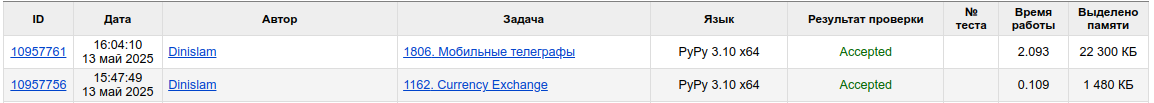
\includegraphics[width=1\textwidth]{check_status.png}
    \caption{Результат проверки}
\end{figure}

\end{document}

